\documentclass[preprint,12pt,authoryear]{elsarticle}
\usepackage[T1]{fontenc}
\usepackage{amsmath,amssymb,booktabs,graphicx,xspace,url}
\usepackage{setspace}
\usepackage[hidelinks]{hyperref}
\makeatletter\g@addto@macro\UrlBreaks{\do\_\do\/\do\.}\makeatother
% generated by reproducibility_p2/scripts/P2_numbers.py -- do not edit
\newcommand{\nDaysFive}{4,495\xspace}
\newcommand{\nEventsFive}{151\xspace}
\newcommand{\EpisFive}{24\xspace}
\newcommand{\EpisTwenty}{16\xspace}
\newcommand{\EpisEraFive}{34\xspace}
\newcommand{\EpisEraTwenty}{22\xspace}
\newcommand{\EpisMin}{9\xspace}
\newcommand{\EpisMax}{34\xspace}
\newcommand{\FirstOOSEra}{1957\xspace}
\newcommand{\FirstOOSBTC}{2018\xspace}
\newcommand{\FirstOOSETH}{2021\xspace}
\newcommand{\HolmMinExp}{\ensuremath{0.084}\xspace}
\newcommand{\MCSfam}{8\xspace}
\newcommand{\GWmax}{\ensuremath{0.0044}\xspace}
\newcommand{\HolmRoll}{\ensuremath{0.015}\xspace}
\newcommand{\SpearmanFive}{\ensuremath{0.998}\xspace}
\newcommand{\SpearmanTwenty}{\ensuremath{0.994}\xspace}
\newcommand{\MCBownFive}{\ensuremath{0.0023}\xspace}
\newcommand{\MCBoperFive}{\ensuremath{0.0131}\xspace}
\newcommand{\MCBownTwenty}{\ensuremath{0.0054}\xspace}
\newcommand{\MCBoperTwenty}{\ensuremath{0.0212}\xspace}
\newcommand{\MCBrawFive}{\ensuremath{0.050}\xspace}
\newcommand{\DSCrawTwenty}{\ensuremath{0.0144}\xspace}
\newcommand{\DSCseqTwenty}{\ensuremath{0.0069}\xspace}
\newcommand{\dDSCseqLo}{\ensuremath{0.0010}\xspace}
\newcommand{\dDSCseqHi}{\ensuremath{0.0144}\xspace}
\newcommand{\ChiFive}{\ensuremath{7\times10^{-4}}\xspace}
\newcommand{\PermFive}{\ensuremath{0.91}\xspace}
\newcommand{\PermMin}{\ensuremath{0.36}\xspace}
\newcommand{\DispFive}{\ensuremath{8.8}\xspace}
\newcommand{\IsoTwenty}{\ensuremath{0.094}\xspace}
\newcommand{\SeqTwenty}{\ensuremath{0.085}\xspace}
\newcommand{\LeadEleven}{2\xspace}
\newcommand{\LeadTwentyTwenty}{2\xspace}
\newcommand{\LeadTwentyFive}{12\xspace}
\newcommand{\SatEleven}{29\xspace}
\newcommand{\SatElevenHit}{2\xspace}
\newcommand{\AlarmElevenDate}{4 August 2011\xspace}
\newcommand{\EntryElevenDate}{8 August 2011\xspace}
\newcommand{\BSSrawEraFive}{\ensuremath{-8.3}\xspace}
\newcommand{\PermEraFive}{\ensuremath{0.37}\xspace}
\newcommand{\QBEraFive}{\ensuremath{0.013}\xspace}
\newcommand{\LabelRows}{500\xspace}
\newcommand{\LabelFromDate}{30 December 2002\xspace}
\newcommand{\LabelToDate}{22 December 2004\xspace}
\newcommand{\NoutB}{4,158\xspace}
\newcommand{\MeanSoutB}{\ensuremath{0.051}\xspace}
\newcommand{\RateOperOutB}{\ensuremath{0.014}\xspace}
\newcommand{\DSCownFive}{\ensuremath{0.0103}\xspace}
\newcommand{\DSCoperFive}{\ensuremath{0.0010}\xspace}
\newcommand{\QBEraTwenty}{\ensuremath{0.033}\xspace}
\newcommand{\PermEraTwenty}{\ensuremath{0.67}\xspace}
\newcommand{\dDSCLogLo}{\ensuremath{0.0006}\xspace}
\newcommand{\dDSCLogHi}{\ensuremath{0.0070}\xspace}
\newcommand{\dDSCGbtLo}{\ensuremath{-0.0009}\xspace}
\newcommand{\dDSCGbtHi}{\ensuremath{0.0064}\xspace}
\newcommand{\GbtZeroBlockTwenty}{40\xspace}
\newcommand{\GbtZeroBlockFive}{none\xspace}
\newcommand{\BSSsFive}{\ensuremath{0.086}\xspace}
\newcommand{\BSSouFive}{\ensuremath{0.119}\xspace}
\newcommand{\dBSSsFive}{\ensuremath{-0.033}\xspace}
\newcommand{\dBSSsFiveLo}{\ensuremath{-0.068}\xspace}
\newcommand{\dBSSsFiveHi}{\ensuremath{0.001}\xspace}
\newcommand{\pEWCsFive}{\ensuremath{0.18}\xspace}
\newcommand{\BSSsTwenty}{\ensuremath{0.086}\xspace}
\newcommand{\BSSouTwenty}{\ensuremath{0.085}\xspace}
\newcommand{\dBSSsTwenty}{\ensuremath{0.001}\xspace}
\newcommand{\dBSSsTwentyLo}{\ensuremath{-0.021}\xspace}
\newcommand{\dBSSsTwentyHi}{\ensuremath{0.029}\xspace}
\newcommand{\pEWCsTwenty}{\ensuremath{0.94}\xspace}
\newcommand{\GWslopeMin}{\ensuremath{0.058}\xspace}
\newcommand{\GWslopeMax}{\ensuremath{0.093}\xspace}
\newcommand{\GWconstMax}{\ensuremath{0.022}\xspace}
\newcommand{\GRcrit}{\ensuremath{3.07}\xspace}
\newcommand{\GRreject}{2\xspace}
\newcommand{\GRmaxExp}{\ensuremath{2.73}\xspace}
\newcommand{\SizeChiFive}{92.5\%\xspace}
\newcommand{\PowChiFive}{93.8\%\xspace}
\newcommand{\SizePermFive}{4.2\%\xspace}
\newcommand{\PowPermFive}{5.7\%\xspace}
\newcommand{\SizeQBFive}{6.6\%\xspace}
\newcommand{\PowQBFive}{8.0\%\xspace}
\newcommand{\SizeChiTwenty}{99.7\%\xspace}
\newcommand{\PowChiTwenty}{99.9\%\xspace}
\newcommand{\SizePermTwenty}{5.3\%\xspace}
\newcommand{\PowPermTwenty}{7.0\%\xspace}
\newcommand{\SizeQBTwenty}{11.9\%\xspace}
\newcommand{\PowQBTwenty}{14.2\%\xspace}
\newcommand{\SimYearsFive}{9\xspace}
\newcommand{\SimEpisFive}{28\xspace}
\newcommand{\PenRawFive}{\ensuremath{0.0034}\xspace}
\newcommand{\PenClimFive}{\ensuremath{0.0026}\xspace}
\newcommand{\PenOthLoFive}{\ensuremath{0.0036}\xspace}
\newcommand{\PenOthHiFive}{\ensuremath{0.0064}\xspace}
\newcommand{\PenRawTwenty}{\ensuremath{0.0135}\xspace}
\newcommand{\PenClimTwenty}{\ensuremath{0.0159}\xspace}
\newcommand{\PenOthLoTwenty}{\ensuremath{0.0169}\xspace}
\newcommand{\PenOthHiTwenty}{\ensuremath{0.0205}\xspace}
\newcommand{\AUCyrRawFive}{\ensuremath{0.83}\xspace}
\newcommand{\AUCyrGbtFive}{\ensuremath{0.88}\xspace}
\newcommand{\AUCyrLogFive}{\ensuremath{0.85}\xspace}
\newcommand{\AUCyrRawTwenty}{\ensuremath{0.73}\xspace}
\newcommand{\AUCyrGbtTwenty}{\ensuremath{0.70}\xspace}
\newcommand{\AUCyrLogTwenty}{\ensuremath{0.71}\xspace}
\newcommand{\SetMaxChange}{\ensuremath{0.042}\xspace}
\newcommand{\ClimEleven}{\ensuremath{0.043}\xspace}
\newcommand{\SeqMaxEleven}{\ensuremath{0.26}\xspace}
\newcommand{\SeqMultEleven}{\ensuremath{6}\xspace}
\newcommand{\GbtMaxEleven}{\ensuremath{0.42}\xspace}
\newcommand{\GbtMultEleven}{\ensuremath{10}\xspace}
\newcommand{\EntriesEleven}{1\xspace}
\newcommand{\ClimTwentyTwenty}{\ensuremath{0.030}\xspace}
\newcommand{\SeqMaxTwentyTwenty}{\ensuremath{0.25}\xspace}
\newcommand{\SeqMultTwentyTwenty}{\ensuremath{8}\xspace}
\newcommand{\GbtMaxTwentyTwenty}{\ensuremath{0.25}\xspace}
\newcommand{\GbtMultTwentyTwenty}{\ensuremath{9}\xspace}
\newcommand{\SatTwentyTwenty}{12\xspace}
\newcommand{\SatTwentyTwentyHit}{3\xspace}
\newcommand{\AlarmTwentyTwentyDate}{25 February 2020\xspace}
\newcommand{\EntryTwentyTwentyDate}{27 February 2020\xspace}
\newcommand{\EntriesTwentyTwenty}{2\xspace}
\newcommand{\ClimTwentyFive}{\ensuremath{0.036}\xspace}
\newcommand{\SeqMaxTwentyFive}{\ensuremath{0.28}\xspace}
\newcommand{\SeqMultTwentyFive}{\ensuremath{8}\xspace}
\newcommand{\GbtMaxTwentyFive}{\ensuremath{0.31}\xspace}
\newcommand{\GbtMultTwentyFive}{\ensuremath{9}\xspace}
\newcommand{\SatTwentyFive}{15\xspace}
\newcommand{\SatTwentyFiveHit}{6\xspace}
\newcommand{\AlarmTwentyFiveDate}{19 March 2025\xspace}
\newcommand{\EntryTwentyFiveDate}{4 April 2025\xspace}
\newcommand{\EntriesTwentyFive}{3\xspace}
% every result number, written by reproducibility_p2/scripts/P2_numbers.py
\newcommand{\fittable}[1]{\begingroup\setbox0=\hbox{#1}\ifdim\wd0>\textwidth\resizebox{\textwidth}{!}{\box0}\else\box0\fi\endgroup}
\newcommand{\Sraw}{S}
\setlength{\emergencystretch}{1.5em}
% ---- submission metadata: the Zenodo DOI placeholder is intentionally unused in this double-blind
% version; it will be filled when the archive is deposited after acceptance.
\newcommand{\ZenodoDOI}{10.5281/zenodo.23491759}
\journal{International Journal of Forecasting}
\begin{document}
\begin{frontmatter}
\title{What does a committor score forecast? Hitting-probability warnings of market stress, their target and their evaluation}
\author[math]{Boyan Xing\corref{cor1}}\ead{t330025089@mail.bnbu.edu.cn}
\author[acc]{Jiayi Pan}
\cortext[cor1]{Corresponding author.}
\affiliation[math]{organization={Department of Mathematical Sciences, Faculty of Science and Technology, Beijing Normal-Hong Kong Baptist University}, city={Zhuhai}, state={Guangdong}, country={China}}
\affiliation[acc]{organization={Department of Accounting, Faculty of Business and Management, Beijing Normal-Hong Kong Baptist University}, city={Zhuhai}, state={Guangdong}, country={China}}
\begin{abstract}
Hitting probabilities computed from fitted or learned dynamics---committor-type scores---are increasingly proposed as early warnings of abrupt transitions in the atmosphere, the climate and markets. We ask what such a score forecasts and how it should be evaluated, using as a case study a committor score of stress in the S\&P~500 that is built from a two-dimensional state of trailing-window features and re-estimated every year from 2008 to 2026. Within each year the score is almost exactly a monotone function of a single linear stress index, and it is close to calibrated for the event it is built to forecast---entry of the state into its own learned stress region---but not for the operational event, a rule-based entry into market stress. After strictly sequential recalibration it cannot be distinguished from the stress index recalibrated in the same way, from logistic regression or from gradient boosting on the same state: daily data contain only \EpisMin to \EpisMax independent stress episodes per sample, and a model confidence set retains the committor forecast in every comparison. An in-sample discrimination advantage of the raw score at 20 days is specific to 2008--2026. An apparent drift of the score's probability meaning across annual re-estimations disappears once dependent days are grouped into episodes; in simulations that copy the data, the day-level test behind the apparent drift rejects a true null in \SizeChiFive of samples. Warning scores of this kind should be evaluated against an explicitly stated target, with inference at the level of episodes.
\end{abstract}
\begin{keyword}
probability forecasting \sep Brier score decomposition \sep early warning \sep forecast comparison \sep model confidence set \sep financial stress
\end{keyword}
\end{frontmatter}
\doublespacing

\section{Introduction}
On \AlarmElevenDate a committor score of stress in the S\&P~500---the probability, computed from a fitted stochastic model, that the market state reaches a stress region within five trading days---exceeded 0.99, and the market entered stress on \EntryElevenDate. Between July and November 2011 the same score exceeded 0.99 on \SatEleven trading days outside the stress set; only \SatElevenHit of them were followed by an entry within five days. Numbers of this kind look like probabilities. This paper asks what such a number forecasts, and how a forecaster should evaluate it.

A growing class of early warnings reports the probability, under fitted or learned dynamics, that a system reaches a learned region of its state space: committor functions for rare transitions in the atmosphere \citep{finkel2021,miloshevich2023} and in climate models \citep{lucente2022}, and hitting probabilities of stress regions in markets. They extend a long tradition of indicators of proximity to a critical transition in ecosystems, the climate and finance \citep{scheffer2009,dakos2012}. A committor, or its finite-horizon version, the hitting probability, is the probability that a Markov process started at the current state reaches a target set before another set or before a time limit \citep{e2010}. When the dynamics are estimated from data and the target set is chosen from the data, the number differs from an operational probability forecast in three ways. Its target is a region of the model's own state space, not necessarily the event a user cares about. It changes whenever the model is re-estimated, so the meaning of a given value may change too. And its evaluation rests on rare events that cluster in time, so that the effective sample is the number of distinct episodes, not the number of days.

We study these three gaps on a case study, a committor-type stress score built on the trailing-window state whose irreversibility and information content the companion paper analyses \citep{xingpan2026}: seven trailing-window features of prices and volumes, reduced to two principal components, an Ornstein--Uhlenbeck (OU) model fitted to them, and a target set equal to the upper decile of a learned stress direction. Re-estimated every year from 2008 to 2026, the score is compared with estimators that use the same information---the stress index itself, a Markov-state model, an analogue Markov chain, logistic regression and gradient boosting---for the first entry into a rule-based stress set within 5 and 20 trading days. The exercise is repeated on an era the protocol has never seen (1957--1999) and on two cryptocurrencies.

The paper makes three contributions to the evaluation of warnings of this kind, none of which depends on the committor construction. First, a diagnosis of target mismatch: the CORP decomposition of the Brier score \citep{dimitriadis2021}, applied once against the score's own target and once against the operational event, separates a score that is miscalibrated because its dynamics are wrong from one that forecasts a different event (Section~\ref{sec:what}). Second, inference at the level of episodes: tests that treat dependent days as independent manufacture drift in the probability meaning of a score, and a simulation that copies the data shows how much---the day-level test rejects a true null in \SizeChiFive of samples, whereas a permutation test with episodes as units holds its nominal size (Section~\ref{sec:drift}). Third, forecast comparison with few episodes: fixed-smoothing Diebold--Mariano tests \citep{lazarus2018,coroneo2020}, the model confidence set \citep{hansen2011} and the conditional test of \citet{giacomini2006} on a finite-memory version of the forecasts, with bootstrap blocks tied to the forecast horizon (Section~\ref{sec:compare}).

For the committor score the findings are clear. Within each year it is almost exactly a monotone function of a single linear stress index, and it is close to calibrated for entry into its learned region but not for the operational event (Section~\ref{sec:what}). Its raw values are dominated by miscalibration; sequential recalibration removes it, and what remains cannot be distinguished from the recalibrated stress index or from simple classifiers on the same state (Sections~\ref{sec:murphy} and~\ref{sec:compare}). An apparent drift of its probability meaning is an artefact of day-level tests (Section~\ref{sec:drift}), and an in-sample discrimination advantage of the raw score at 20 days does not transfer to other samples (Section~\ref{sec:markets}). Behind all of these lies one constraint: daily data on market stress contain between \EpisMin and \EpisMax independent event episodes per sample. Four practices follow for any score of proximity to a learned region (Section~\ref{sec:discussion}): state the target; do not pool AUCs of forecasts recalibrated year by year; carry out inference at the level of episodes; and, when the Giacomini--White test is used, evaluate a finite-memory version of the forecasts alongside the expanding one.

The evaluation draws on the decomposition of probability scores \citep{murphy1973,stephenson2008,brocker2009,dimitriadis2021} and its graphical form, the triptych of Murphy, reliability and ROC diagrams \citep{dimitriadis2024}, on proper scoring rules and calibration \citep{gneiting2007scoring,gneiting2007calibration}, on tests of equal predictive ability \citep{diebold1995,harvey1997,giacomini2006,diebold2015} with fixed-smoothing variance estimates \citep{lazarus2018,coroneo2020}, on comparisons under instability \citep{giacomini2010}, and on the model confidence set \citep{hansen2011}. Early-warning systems for financial crises are judged by signal-to-noise ratios or policy-weighted losses \citep{kaminsky1998,alessi2011,drehmann2014}, within unified statistical frameworks \citep{candelon2012} and dynamic models \citep{candelon2014}, and by horse races of classifiers and machine learning \citep{holopainen2017,beutel2019,fouliard2021,bluwstein2023}; committor forecasts in geophysics are judged by proper scores \citep{finkel2021,miloshevich2023}. The companion paper analyses what trailing windows do to the irreversibility and information content of the state \citep{xingpan2026}; here the forecasts are taken as given and the question is what they predict.

\section{Data, event and forecasts}\label{sec:data}
\paragraph{Data.} The data and the seven features are those of the companion paper \citep[Appendix~E]{xingpan2026}; we list what matters for forecasting. Daily closing prices and volumes of the S\&P~500 (\textasciicircum GSPC) run from 3 January 2000 to 16 October 2026; the one zero volume in Yahoo's record (24 May 2023) is filled from a second vendor (Appendix~\ref{app:data}). The era test uses an independent Yahoo-derived archive for 1950--1999 \citep{vijinho}, and the cryptocurrency tests use Coin Metrics prices and reported spot volumes of Bitcoin and Ether \citep{coinmetrics}.

\paragraph{Operational event.} The stress set is the rule of the protocol: 20-day realized volatility above its lagged 1000-day 85\% quantile and a 20-day drawdown below $-8\%$ ($-15\%$ for the cryptocurrencies). The event at horizon $h$ is the first entry into the set within $(t,t+h]$, $h\in\{5,20\}$ trading days, and days already in the set are not scored, much as crisis and post-crisis periods are set apart in the crisis-prediction literature \citep{bussiere2006}. In 2008--2026 there are \nEventsFive event days among \nDaysFive scored days at $h=5$, and they form only \EpisFive \emph{event episodes}---groups of event days no more than $h$ trading days apart (Table~\ref{tab:samples}). \emph{Saturation episodes}, used in Section~\ref{sec:drift}, are formed in the same way from the days on which the raw score exceeds 0.99, and are split at the annual re-estimation.

\paragraph{Committor score.} The state consists of log realized volatility over 20 and 5 days, relative log activity (20-day over 250-day mean volume), the 20-day drawdown and log return, and the rolling 60-day variance and lag-one autocorrelation of differenced log volatility. For each year $Y$ the features before $Y$ are standardized and projected on their first two principal components, which are standardized again, giving $z_t$. Least squares of $z_{t+1}-z_t$ on $z_t$ gives the drift $Az+b$ and the residual covariance $D$ of an OU process. The stress direction $w$ is the unit vector of correlations of the two components with log 20-day volatility, $s_t=w^\top z_t$ is the stress coordinate, and the learned target is $B=\{z: w^\top z\ge q\}$, with $q$ the 90\% training quantile of $s$. The score
\begin{equation}
\Sraw_t=\Pr\nolimits_{\rm OU}\left(\tau_B\le h \mid Z_0=z_t\right)
\end{equation}
is computed by implicit Euler steps of the backward Kolmogorov equation on a $40\times40$ grid. It is a probability by construction---of the event that the fitted process enters $B$ within $h$ days.

\paragraph{Matched estimators.} On the same state and labels we fit a Markov-state model with 100 $k$-means states and $B$ absorbing \citep{prinz2011}, the analogue Markov chain of \citet{lucente2022} with 20 analogues, logistic regression (ridge penalty with $C=1$ on the two components and $C=0.2$ on the seven standardized features) and gradient-boosted trees \citep{friedman2001} (depth 2, 120 trees, learning rate 0.03, at least 20 observations per leaf) on the two components and on the seven features. The settings are fixed in advance; Table~\ref{tab:settings} reports logistic regression with $C\in\{0.1,1,10\}$ and boosting tuned by time-series cross-validation over depth and number of trees, which change the Brier skill by at most \SetMaxChange. The three dynamical scores (OU, MSM, AMC) and the stress coordinate $s$ itself are recalibrated strictly sequentially by a logistic regression of past labels on past out-of-sample scores, with the training climatology until at least 100 past observations, 5 events and 20 non-events exist (seq-cal).

\paragraph{Evaluation.} Models are re-estimated on annual expanding windows, 2008--2026; a rolling five-year variant, for estimation and for the recalibration memory, provides the finite-memory setting of the Giacomini--White test. Every result is reported with and without 2008, the cold-start year in which seq-cal falls back to climatology in the middle of the largest crisis. Forecasts are scored by the Brier score (BS) and its skill (BSS) against the year-specific training climatology, and BS is decomposed as
\begin{equation}
{\rm BS}={\rm MCB}-{\rm DSC}+{\rm UNC},\qquad {\rm MCB}={\rm BS}(p)-{\rm BS}(\hat p),\quad {\rm DSC}={\rm UNC}-{\rm BS}(\hat p),
\end{equation}
where $\hat p$ is the isotonic (PAV) recalibration of $p$ and UNC the base-rate uncertainty \citep{dimitriadis2021}: DSC is the discrimination a single monotone recalibration would realize, MCB the cost of not doing it. AUC is reported only for raw scores and classifiers; the pooled AUC of a forecast recalibrated year by year, or of climatology, mixes calibration levels across years and does not measure discrimination (within-year AUCs are in Table~\ref{tab:auc}). Intervals come from a moving-block bootstrap \citep{kunsch1989} with blocks of $2h$ trading days, so that a block spans two overlapping label windows (10 days at $h=5$, 40 at $h=20$); we tie the block to the horizon rather than use an automatic choice \citep{politis2004}, and Table~\ref{tab:blocks} reports blocks of 5 to 60 days. Unconditional tests use equal-weighted-cosine fixed-smoothing variances \citep{lazarus2018} with Holm adjustment over comparators \citep{holm1979}; the conditional test of \citet{giacomini2006} uses the last observed loss differential as instrument; and the model confidence set \citep{hansen2011} uses the $T_{\max}$ statistic at the 10\% level (Appendix~\ref{app:inference}).

\section{What the score forecasts}\label{sec:what}
Within each year the committor score is a monotone function of one linear stress index, and it forecasts entry into its own learned region rather than the operational event. The median within-year Spearman correlation between $\Sraw$ and the stress coordinate $s$ is \SpearmanFive at 5 days and \SpearmanTwenty at 20 days [Fig.~\ref{fig:anatomy}(a)]. The fitted two-dimensional dynamics therefore add almost nothing to the ordering of days beyond the projection on the learned direction, and the AUCs of $\Sraw$ and of $s$ for the operational event differ by amounts whose bootstrap intervals include zero at both horizons. Recalibrating $s$ itself with the same sequential map shows what they add to the forecast. At 20 days nothing: the Brier skill is \BSSsTwenty against \BSSouTwenty for the recalibrated committor score, a difference of \dBSSsTwenty [\dBSSsTwentyLo, \dBSSsTwentyHi]. At 5 days the recalibrated index is less skilful (\BSSsFive against \BSSouFive; difference \dBSSsFive [\dBSSsFiveLo, \dBSSsFiveHi], EWC $p=\,$\pEWCsFive), and the whole difference is calibration: the two forecasts discriminate equally, but the nonlinear map from $s$ to $\Sraw$ suits the logistic recalibration better than $s$ itself (Tables~\ref{tab:corp} and~\ref{tab:dbss}). In the terms of the companion paper, the current that the fitted OU model carries in its plane---mostly the leverage effect---does not change which days the score ranks as most stressed.

What the score is calibrated for is its own target. On the \NoutB scored days outside the learned region (days in the region, where the score saturates, excluded), the miscalibration term of $\Sraw$ against entry into that region is \MCBownFive at 5 days and \MCBownTwenty at 20 days, against \MCBoperFive and \MCBoperTwenty for the operational event [Fig.~\ref{fig:anatomy}(b,c)]. On all \nDaysFive scored days, where saturated days enter, the miscalibration of the raw score for the operational event is \MCBrawFive (Table~\ref{tab:corp}). Two simpler numbers tell the same story: outside the learned region the mean score at 5 days is \MeanSoutB while the operational event rate is \RateOperOutB, and the score discriminates its own target an order of magnitude better than the operational event (DSC \DSCownFive against \DSCoperFive). The fitted dynamics roughly know their own hitting probabilities; the operational event is rarer and overlaps only partly with entries into the learned region. Most of the miscalibration of the raw score is therefore target mismatch rather than a failure of the dynamics. For a user this means that a committor score must be recalibrated against the event that matters before it is read as a probability, and that a reliability diagram against the score's own target is the quickest way to tell the two failures apart.

\begin{figure}[t]\centering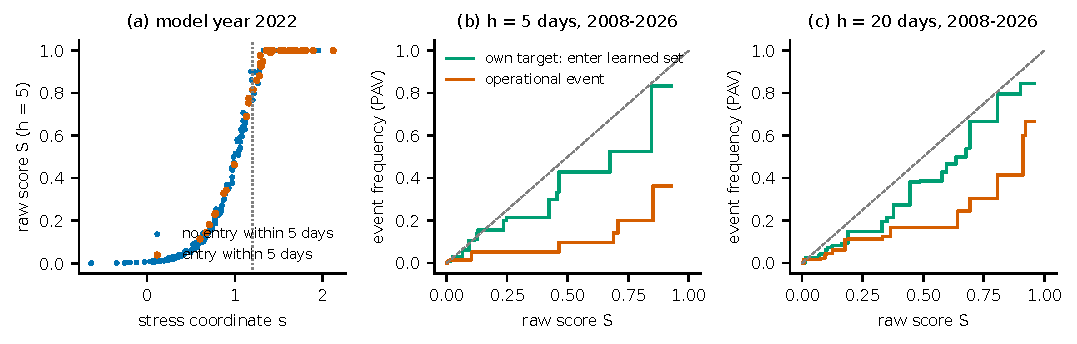
\includegraphics[width=\textwidth]{figures/fig1_anatomy.pdf}
\caption{The committor score is a monotone function of one stress index and is calibrated for its own target. (a) $\Sraw$ against the stress coordinate $s$ in model year 2022 ($h=5$); dotted, threshold of the learned target. (b,c) PAV-recalibrated event frequency against $\Sraw$ on days outside the learned region, for entry into that region and for the operational event, 2008--2026. Data: P2\_F1\_anatomy\_exp.csv, P2\_F6\_own\_target\_exp.csv.}\label{fig:anatomy}\end{figure}

\section{Resolution and reliability}\label{sec:murphy}
The raw score discriminates about as well as the best estimator on the same state but is almost useless as a probability; sequential recalibration repairs the probability and gives up part of the discrimination. Miscalibration dominates the raw score: its MCB term at 5 days is \MCBrawFive, an order of magnitude larger than its discrimination, so its skill is strongly negative (Table~\ref{tab:corp}, Fig.~\ref{fig:corp}). Recalibration brings MCB down to the level of the classifiers.

Discrimination needs a closer look. At 20 days the DSC of the raw score in 2008--2026 is \DSCrawTwenty, against \DSCseqTwenty after recalibration, and the paired bootstrap interval of the difference, [\dDSCseqLo, \dDSCseqHi], excludes zero. The comparison is not between equals. CORP measures the discrimination of every forecast after the single monotone (PAV) map that is optimal over the whole sample, so the DSC of the raw score is the discrimination it would reach if that in-sample map were known: an upper bound, not a realizable forecast. Within a year the recalibrated forecast is a fixed increasing transform of the raw score and orders days identically, so the difference arises entirely across years. There one global map is optimal, because there is no evidence that the probability meaning of the score drifts (Section~\ref{sec:drift}), whereas the sequential map, re-estimated every year from few past episodes, discards information while the history is short. The achievable gap is that of a real-time monotone recalibrator: isotonic recalibration on past scores reaches a Brier skill of \IsoTwenty at 20 days against \SeqTwenty for the logistic map. In the same in-sample sense the raw score discriminates better than logistic regression on the two components ([\dDSCLogLo, \dDSCLogHi]), while gradient boosting cannot be distinguished from it ([\dDSCGbtLo, \dDSCGbtHi]), and the ordering survives the exclusion of 2008. At 5 days the raw score has no such advantage, and gradient boosting discriminates better when 2008 is included. Section~\ref{sec:markets} shows that the in-sample advantage at 20 days is specific to 2008--2026. For a user, the raw score is worth recalibrating rather than replacing, but a better real-time recalibrator buys little.

\begin{table}[t]\centering\small
\caption{CORP decomposition of the Brier score, S\&P~500 (BS $=$ MCB $-$ DSC $+$ UNC). AUC is not defined as a discrimination measure for sequentially recalibrated forecasts and is not shown for them.}\label{tab:corp}
\fittable{\begin{tabular}{lrrrrrrrr}\toprule
 & \multicolumn{4}{c}{$h=5$ days} & \multicolumn{4}{c}{$h=20$ days}\\
\cmidrule(lr){2-5}\cmidrule(lr){6-9} method & BSS & MCB & DSC & AUC & BSS & MCB & DSC & AUC\\\midrule
\multicolumn{9}{l}{\emph{2008--2026}}\\
OU raw S & $-1.321$ & $0.0497$ & $0.0058$ & $0.918$ & $-0.319$ & $0.0437$ & $0.0144$ & $0.814$\\
OU seq-cal & $0.119$ & $0.0006$ & $0.0041$ & -- & $0.085$ & $0.0024$ & $0.0069$ & --\\
stress index $s$ seq-cal & $0.086$ & $0.0018$ & $0.0042$ & -- & $0.086$ & $0.0018$ & $0.0064$ & --\\
MSM seq-cal & $0.115$ & $0.0006$ & $0.0039$ & -- & $0.064$ & $0.0032$ & $0.0059$ & --\\
AMC seq-cal & $0.119$ & $0.0007$ & $0.0041$ & -- & $0.066$ & $0.0033$ & $0.0063$ & --\\
PC2 logistic & $0.102$ & $0.0027$ & $0.0056$ & $0.890$ & $0.127$ & $0.0024$ & $0.0105$ & $0.752$\\
PC2 GBT & $0.195$ & $0.0009$ & $0.0069$ & $0.877$ & $0.151$ & $0.0017$ & $0.0118$ & $0.735$\\
raw logistic & $0.097$ & $0.0009$ & $0.0036$ & $0.833$ & $0.093$ & $0.0020$ & $0.0072$ & $0.722$\\
raw GBT & $0.116$ & $0.0022$ & $0.0056$ & $0.848$ & $0.105$ & $0.0051$ & $0.0113$ & $0.719$\\
\multicolumn{9}{l}{\emph{2009--2026 (without 2008)}}\\
OU raw S & $-1.115$ & $0.0348$ & $0.0047$ & $0.920$ & $-0.355$ & $0.0368$ & $0.0103$ & $0.795$\\
OU seq-cal & $0.152$ & $0.0006$ & $0.0045$ & -- & $0.104$ & $0.0020$ & $0.0082$ & --\\
stress index $s$ seq-cal & $0.110$ & $0.0018$ & $0.0046$ & -- & $0.105$ & $0.0012$ & $0.0075$ & --\\
MSM seq-cal & $0.147$ & $0.0006$ & $0.0043$ & -- & $0.079$ & $0.0027$ & $0.0071$ & --\\
AMC seq-cal & $0.153$ & $0.0007$ & $0.0046$ & -- & $0.082$ & $0.0029$ & $0.0075$ & --\\
PC2 logistic & $0.073$ & $0.0023$ & $0.0040$ & $0.897$ & $0.096$ & $0.0016$ & $0.0072$ & $0.742$\\
PC2 GBT & $0.181$ & $0.0007$ & $0.0053$ & $0.901$ & $0.125$ & $0.0015$ & $0.0092$ & $0.746$\\
raw logistic & $0.063$ & $0.0009$ & $0.0024$ & $0.847$ & $0.072$ & $0.0019$ & $0.0057$ & $0.743$\\
raw GBT & $0.113$ & $0.0022$ & $0.0051$ & $0.882$ & $0.083$ & $0.0051$ & $0.0098$ & $0.765$\\
\bottomrule\end{tabular}
}\end{table}

\begin{figure}[t]\centering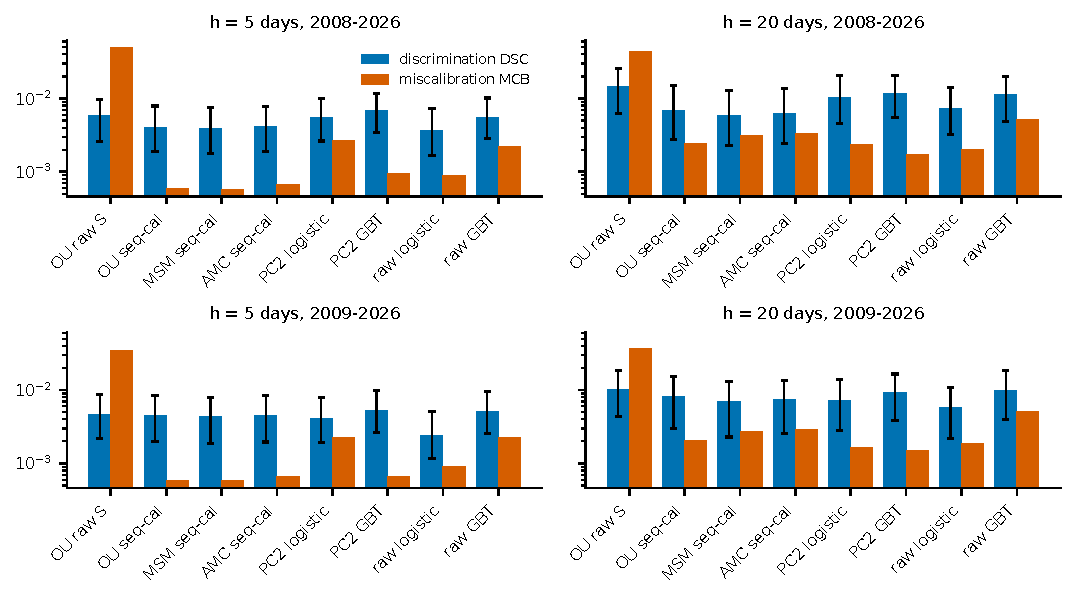
\includegraphics[width=\textwidth]{figures/fig2_corp.pdf}
\caption{Miscalibration dominates the raw score; discrimination is comparable across estimators. CORP terms on a log scale; error bars, 90\% moving-block-bootstrap intervals of DSC (blocks of $2h$ days). Data: P2\_F2\_decomposition\_exp.csv, P2\_F2\_bootstrap\_exp.csv.}\label{fig:corp}\end{figure}

\section{Does the probability meaning drift?}\label{sec:drift}
The event frequency on days with a saturated score varies widely between years, but no more than expected when days come in episodes. A natural test of drift compares the event rate on days with $\Sraw>0.99$ across model years. A chi-square test that treats these days as independent rejects homogeneity ($p=\,$\ChiFive at 5 days, and more strongly at 20 days). Saturated days, however, come in runs that share their future---the forecast horizons overlap---and their episode. Grouping them into saturation episodes and permuting year labels across whole episodes \citep{ernst2004} gives $p=\,$\PermFive at 5 days (Table~\ref{tab:drift}, Fig.~\ref{fig:saturation}). Across both horizons, both window schemes and three cluster definitions, and with a quasi-binomial test on episode counts \citep{mccullagh1989}, no $p$-value falls below \PermMin. The estimated dispersion, \DispFive at 5 days, measures how far the days are from independent: a saturated episode carries roughly the information of one observation, whatever its length.

Real-time recalibrators that could adapt to drift do not help either. Mapping $\Sraw$ through its rank among the model's own training scores, or through the rank of the stress coordinate, lowers the skill, and isotonic recalibration improves it only slightly at 20 days (BSS \IsoTwenty against \SeqTwenty). An annual standardization of $\operatorname{logit}\Sraw$ that uses each test year's own mean and spread---an ex post transform reported for completeness---does worst. The drift penalty, the gain in discrimination from allowing one monotone map per year instead of one for all years (Appendix~\ref{app:inference}), makes the last point quantitative. At 5 days it is \PenRawFive for the raw score and between \PenOthLoFive and \PenOthHiFive for the other forecasts, while climatology, which is constant within each year, gains \PenClimFive from the year-to-year variation of the base rate alone; at 20 days the corresponding numbers are \PenRawTwenty, \PenOthLoTwenty--\PenOthHiTwenty and \PenClimTwenty. The probability meaning of the committor score therefore changes across re-estimations no more than that of any forecast on the same state.

\subsection{How often do day-level tests find drift that is not there?}\label{sec:size}
To see how much the day-level test is distorted, we simulate samples that copy the headline sample at each horizon---\SimYearsFive model years with at least five saturated days and \SimEpisFive saturation episodes at $h=5$---under a true null of a constant probability that an episode is followed by an operational entry. Each episode has a geometric number of saturated days, and with the common probability it is followed by an entry at a random time within the episode or the $h$ days after it; days are labelled and dropped from scoring as in the data (Appendix~\ref{app:inference}). Table~\ref{tab:size} reports rejection rates at the 5\% level. The day-level chi-square rejects the true null in \SizeChiFive of samples at 5 days and \SizeChiTwenty at 20 days: with dependent days it is not a test. The episode permutation test holds its size (\SizePermFive and \SizePermTwenty), while the quasi-binomial test is liberal (\SizeQBFive and \SizeQBTwenty), as its common dispersion is estimated from few episodes. When the odds of an entry vary across years with a standard deviation of one on the logit scale ($\delta=1$), the permutation test detects it in only \PowPermFive of samples at 5 days and \PowPermTwenty at 20 days. A significant day-level test is thus expected under no drift at all, and with \SimYearsFive model years and a few dozen episodes even substantial drift is almost undetectable: the absence of evidence for drift in Table~\ref{tab:drift} is not evidence of stability.

\begin{table}[t]\centering\small
\caption{Homogeneity across years of the event rate on days with $\Sraw>0.99$ ($p$-values; number of units in parentheses). The day-level chi-square assumes independent days and is shown only for comparison. Episodes are saturation episodes (Section~\ref{sec:data}).}\label{tab:drift}
\fittable{\begin{tabular}{llrrrr}\toprule
 & & \multicolumn{2}{c}{expanding windows} & \multicolumn{2}{c}{rolling five-year windows}\\
\cmidrule(lr){3-4}\cmidrule(lr){5-6} test & units & $h=5$ & $h=20$ & $h=5$ & $h=20$\\\midrule
chi-square (invalid) & days & $7\times10^{-4}$ (273) & $4\times10^{-8}$ (276) & $3\times10^{-4}$ (362) & $2\times10^{-8}$ (366)\\
cluster permutation & episodes, gap $h$ & 0.91 (28) & 0.66 (15) & 0.87 (39) & 0.85 (20)\\
cluster permutation & episodes, gap $2h$ & 0.89 (24) & 0.46 (10) & 0.79 (29) & 0.62 (15)\\
cluster permutation & 20-day blocks & 0.63 (40) & 0.45 (40) & 0.56 (49) & 0.53 (49)\\
quasi-binomial F & episodes, gap $h$ & 0.90 (28) & 0.69 (15) & 0.83 (39) & 0.76 (20)\\
quasi-binomial F & episodes, gap $2h$ & 0.90 (24) & 0.45 (10) & 0.84 (29) & 0.36 (15)\\
quasi-binomial F & 20-day blocks & 0.69 (40) & 0.36 (40) & 0.62 (49) & 0.38 (49)\\
\bottomrule\end{tabular}
}\end{table}

\begin{table}[t]\centering\small
\caption{Rejection rates at the 5\% level of three tests of homogeneity of the saturated-day event rate, in 2,000 simulated samples that copy the headline sample (Section~\ref{sec:size}); null: constant event probability per saturation episode; $\delta$: standard deviation across years of the log odds. Monte Carlo standard errors are about 0.005 at a rate of 0.05 and at most 0.011. Data: P2\_S1\_size\_simulation.csv (seed 20261027).}\label{tab:size}
\fittable{\begin{tabular}{lrrrrrr}\toprule
 & \multicolumn{3}{c}{$h=5$ days} & \multicolumn{3}{c}{$h=20$ days}\\
\cmidrule(lr){2-4}\cmidrule(lr){5-7} test & null & $\delta=0.5$ & $\delta=1$ & null & $\delta=0.5$ & $\delta=1$\\\midrule
day-level chi-square & 0.925 & 0.938 & 0.938 & 0.997 & 0.997 & 0.999\\
episode permutation & 0.043 & 0.062 & 0.057 & 0.053 & 0.067 & 0.070\\
quasi-binomial F & 0.066 & 0.078 & 0.080 & 0.119 & 0.134 & 0.142\\
\bottomrule\end{tabular}
}\end{table}

\begin{figure}[t]\centering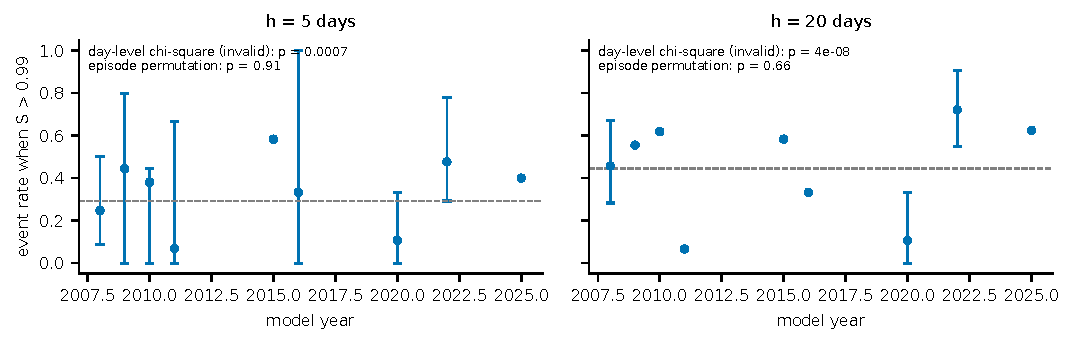
\includegraphics[width=\textwidth]{figures/fig3_saturation.pdf}
\caption{Year-to-year variation of the event rate on saturated days lies within episode-level sampling variation. Error bars, 90\% intervals from resampling whole saturation episodes within the year; dashed, pooled rate. Data: P2\_F3\_saturation\_exp.csv, P2\_F3\_homogeneity\_exp.csv.}\label{fig:saturation}\end{figure}

\section{Matched comparisons}\label{sec:compare}
With the available episodes, no estimator on the same information can be distinguished from the recalibrated committor forecast. The effective sample is small: \EpisFive event episodes at 5 days and \EpisTwenty at 20 days in 2008--2026 (Table~\ref{tab:samples}). Point estimates favour gradient boosting on the two components in every sample and horizon, and the unadjusted bootstrap intervals put the two dynamical alternatives below the OU score at 20 days (Table~\ref{tab:dbss}, Fig.~\ref{fig:compare}). The interval for gradient boosting depends on the block length: at 20 days in 2008--2026 it includes zero for blocks of \GbtZeroBlockTwenty days or more, the headline included, whereas at 5 days in 2008--2026 it excludes zero for every block length from 5 to 60 days; without 2008 it includes zero at both horizons (Table~\ref{tab:blocks}). None of the differences survives a fixed-smoothing test with Holm adjustment in the headline windows; the smallest adjusted $p$-value is \HolmMinExp (Table~\ref{tab:tests}). The model confidence set at the 10\% level contains the committor forecast in all \MCSfam combinations of horizon, sample and window scheme, and excludes climatology in seven of them and logistic regression on the raw features in three (Table~\ref{tab:mcsall}).

The conditional test, whose instrument is the last observed loss differential, rejects equal conditional accuracy of the OU score and its two dynamical siblings at 20 days ($p\le\,$\GWmax in the headline windows). Its statistic contains a constant as well as the lagged differential, and the rejection comes from the constant: tested alone, the lagged differential has $p$-values between \GWslopeMin and \GWslopeMax and the constant at most \GWconstMax (Newey--West variance). The conditional rejection therefore restates a level difference that the more conservative fixed-smoothing test does not confirm after Holm adjustment, rather than showing that the better forecast depends on the last episode. The fluctuation test of \citet{giacomini2010}, which asks whether relative accuracy changes over time, finds no instability in the expanding windows (largest statistic \GRmaxExp against a critical value of \GRcrit) and rejects in \GRreject of the four rolling-window comparisons, both against the analogue Markov chain, where the committor forecast is the more accurate in the most recent windows. In the rolling windows, where the Giacomini--White asymptotics apply formally, logistic regression on the seven raw features is worse than the committor forecast at 20 days without 2008 (adjusted $p=\,$\HolmRoll), the only difference in the study that survives the multiplicity adjustment (Table~\ref{tab:rolling}). For a user the message is that, with this many episodes, the choice among these forecasts is not a statistical question.

\begin{table}[t]\centering\small
\caption{Sample sizes, event days and independent event episodes (event days no more than $h$ trading days apart).}\label{tab:samples}
\fittable{\begin{tabular}{lrrrrrr}\toprule
 & \multicolumn{3}{c}{$h=5$ days} & \multicolumn{3}{c}{$h=20$ days}\\
\cmidrule(lr){2-4}\cmidrule(lr){5-7} sample & days & event days & event episodes & days & event days & event episodes\\\midrule
S\&P 500, 2008--2026 & 4,495 & 151 & 24 & 4,480 & 400 & 16\\
S\&P 500, 2009--2026 & 4,308 & 118 & 19 & 4,293 & 325 & 12\\
S\&P 500, 1957--1999 & 10,576 & 167 & 34 & 10,561 & 536 & 22\\
Bitcoin, 2018--2026 & 2,880 & 84 & 16 & 2,865 & 265 & 11\\
Ether, 2021--2026 & 1,824 & 58 & 11 & 1,809 & 184 & 9\\
\bottomrule\end{tabular}
}\end{table}

\begin{table}[t]\centering\small
\caption{Difference in Brier skill, comparator minus recalibrated committor forecast (positive: comparator better), expanding windows, with 90\% moving-block-bootstrap intervals (blocks of $2h$ days; other block lengths in Table~\ref{tab:blocks}).}\label{tab:dbss}
\fittable{\begin{tabular}{lrrrr}\toprule
comparator & $h=5$, 2008--2026 & $h=5$, 2009--2026 & $h=20$, 2008--2026 & $h=20$, 2009--2026\\\midrule
MSM seq-cal & $-0.004$ & $-0.005$ & $-0.021$ & $-0.026$\\
 & {\scriptsize[-0.015, +0.006]} & {\scriptsize[-0.020, +0.006]} & {\scriptsize[-0.040, -0.005]} & {\scriptsize[-0.050, -0.010]}\\
AMC seq-cal & $0.000$ & $0.000$ & $-0.018$ & $-0.023$\\
 & {\scriptsize[-0.007, +0.006]} & {\scriptsize[-0.009, +0.006]} & {\scriptsize[-0.033, -0.007]} & {\scriptsize[-0.042, -0.011]}\\
PC2 logistic & $-0.017$ & $-0.079$ & $0.043$ & $-0.009$\\
 & {\scriptsize[-0.105, +0.083]} & {\scriptsize[-0.123, -0.021]} & {\scriptsize[-0.021, +0.109]} & {\scriptsize[-0.046, +0.059]}\\
PC2 GBT & $0.076$ & $0.029$ & $0.066$ & $0.021$\\
 & {\scriptsize[+0.006, +0.137]} & {\scriptsize[-0.010, +0.066]} & {\scriptsize[-0.003, +0.114]} & {\scriptsize[-0.018, +0.066]}\\
raw logistic & $-0.022$ & $-0.090$ & $0.009$ & $-0.032$\\
 & {\scriptsize[-0.107, +0.068]} & {\scriptsize[-0.134, -0.033]} & {\scriptsize[-0.052, +0.064]} & {\scriptsize[-0.080, +0.021]}\\
raw GBT & $-0.003$ & $-0.040$ & $0.020$ & $-0.021$\\
 & {\scriptsize[-0.095, +0.079]} & {\scriptsize[-0.130, +0.039]} & {\scriptsize[-0.087, +0.085]} & {\scriptsize[-0.128, +0.079]}\\
stress index $s$ seq-cal & $-0.033$ & $-0.042$ & $0.001$ & $0.001$\\
 & {\scriptsize[-0.068, +0.001]} & {\scriptsize[-0.081, +0.003]} & {\scriptsize[-0.021, +0.029]} & {\scriptsize[-0.024, +0.039]}\\
\bottomrule\end{tabular}
}\end{table}

\begin{table}[t]\centering\small
\caption{Tests against the recalibrated committor forecast, expanding windows: Holm-adjusted fixed-smoothing (EWC) tests of equal accuracy, Giacomini--White conditional tests (Newey--West variance), and model-confidence-set $p$-values (a model is in the 90\% set if its $p$-value is at least 0.10; all eight families in Table~\ref{tab:mcsall}).}\label{tab:tests}
\fittable{\begin{tabular}{lrrrrrr}\toprule
\multicolumn{7}{l}{\emph{$h=5$ days}}\\
 & \multicolumn{3}{c}{2008--2026} & \multicolumn{3}{c}{2009--2026}\\\cmidrule(lr){2-4}\cmidrule(lr){5-7}
comparator & Holm $p$ & GW $p$ & MCS $p$ & Holm $p$ & GW $p$ & MCS $p$\\\midrule
MSM seq-cal & 1.00 & 0.073 & 0.82 & 1.00 & 0.076 & 0.52\\
AMC seq-cal & 1.00 & 0.80 & 0.82 & 1.00 & 0.76 & 0.52\\
PC2 logistic & 1.00 & 0.21 & 0.82 & 0.33 & 0.080 & 0.18\\
PC2 GBT & 0.77 & 0.17 & 1.00 & 1.00 & 0.38 & 1.00\\
raw logistic & 1.00 & 0.16 & 0.76 & 0.26 & 0.039 & 0.085\\
raw GBT & 1.00 & 0.37 & 0.82 & 1.00 & 0.59 & 0.52\\
OU seq-cal (reference) & & & 0.82 & & & 0.52\\\midrule
\multicolumn{7}{l}{\emph{$h=20$ days}}\\
 & \multicolumn{3}{c}{2008--2026} & \multicolumn{3}{c}{2009--2026}\\\cmidrule(lr){2-4}\cmidrule(lr){5-7}
comparator & Holm $p$ & GW $p$ & MCS $p$ & Holm $p$ & GW $p$ & MCS $p$\\\midrule
MSM seq-cal & 0.19 & 0.004 & 0.23 & 0.21 & 0.003 & 0.72\\
AMC seq-cal & 0.084 & 0.003 & 0.27 & 0.089 & 0.001 & 0.76\\
PC2 logistic & 0.88 & 0.42 & 0.65 & 1.00 & 0.87 & 0.91\\
PC2 GBT & 0.54 & 0.13 & 1.00 & 1.00 & 0.005 & 1.00\\
raw logistic & 1.00 & 0.99 & 0.56 & 1.00 & 0.60 & 0.72\\
raw GBT & 1.00 & 0.44 & 0.65 & 1.00 & 0.30 & 0.91\\
OU seq-cal (reference) & & & 0.56 & & & 0.91\\
\bottomrule\end{tabular}
}\end{table}

\begin{figure}[t]\centering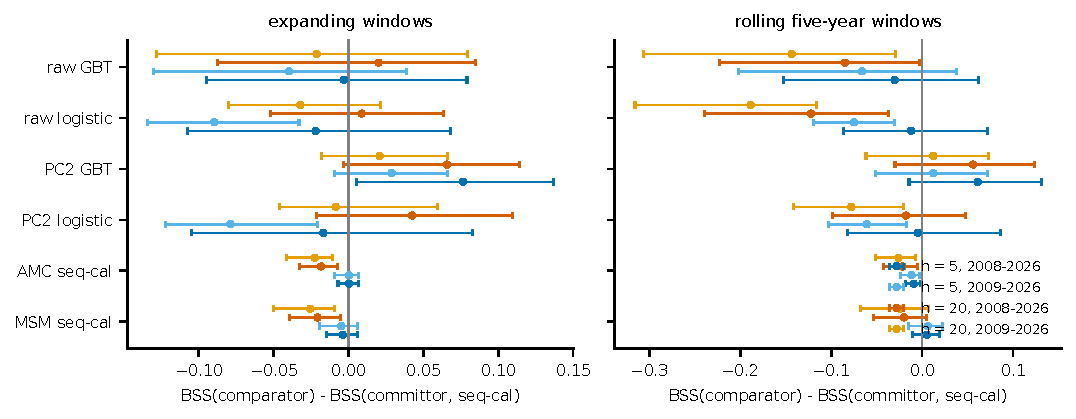
\includegraphics[width=\textwidth]{figures/fig4_comparisons.pdf}
\caption{No estimator can be distinguished from the recalibrated committor forecast after adjustment for multiplicity. Points, difference in BSS; bars, 90\% moving-block-bootstrap intervals (blocks of $2h$ days). Data: P2\_F4\_summary.csv.}\label{fig:compare}\end{figure}

\section{Three episodes}\label{sec:cases}
The score saturates days to weeks before the stress entries of 2011, 2020 and 2025, and it saturates far more often than stress follows (Fig.~\ref{fig:cases}).

\emph{August 2011.} The raw score first exceeded 0.99 on \AlarmElevenDate, \LeadEleven trading days before the first entry on \EntryElevenDate. Over the 20 days before the entry the recalibrated forecast rose to \SeqMaxEleven, \SeqMultEleven times the training climatology of \ClimEleven, and gradient boosting to \GbtMaxEleven (\GbtMultEleven times). Between July and November the raw score was saturated on \SatEleven days outside the stress set, of which only \SatElevenHit were followed by an entry within five days.

\emph{February--March 2020.} The raw score first exceeded 0.99 on \AlarmTwentyTwentyDate, \LeadTwentyTwenty trading days before the first of \EntriesTwentyTwenty entries, on \EntryTwentyTwentyDate. The recalibrated forecast peaked at \SeqMaxTwentyTwenty (\SeqMultTwentyTwenty times climatology) and gradient boosting at \GbtMaxTwentyTwenty (\GbtMultTwentyTwenty times); of \SatTwentyTwenty saturated days outside the set, \SatTwentyTwentyHit were followed by an entry.

\emph{March--April 2025.} Here the alarm came early: the raw score first exceeded 0.99 on \AlarmTwentyFiveDate, \LeadTwentyFive trading days before the first of \EntriesTwentyFive entries, on \EntryTwentyFiveDate. The recalibrated forecast peaked at \SeqMaxTwentyFive (\SeqMultTwentyFive times climatology) and gradient boosting at \GbtMaxTwentyFive (\GbtMultTwentyFive times); \SatTwentyFiveHit of \SatTwentyFive saturated days were followed by an entry.

In all three episodes the recalibrated forecast and gradient boosting rose to several times the training climatology over the same days, without approaching one, and neither led the other systematically. A saturated committor score says that the state is at or beyond the boundary of the learned region; it does not say that the operational event is near.

\begin{figure}[t]\centering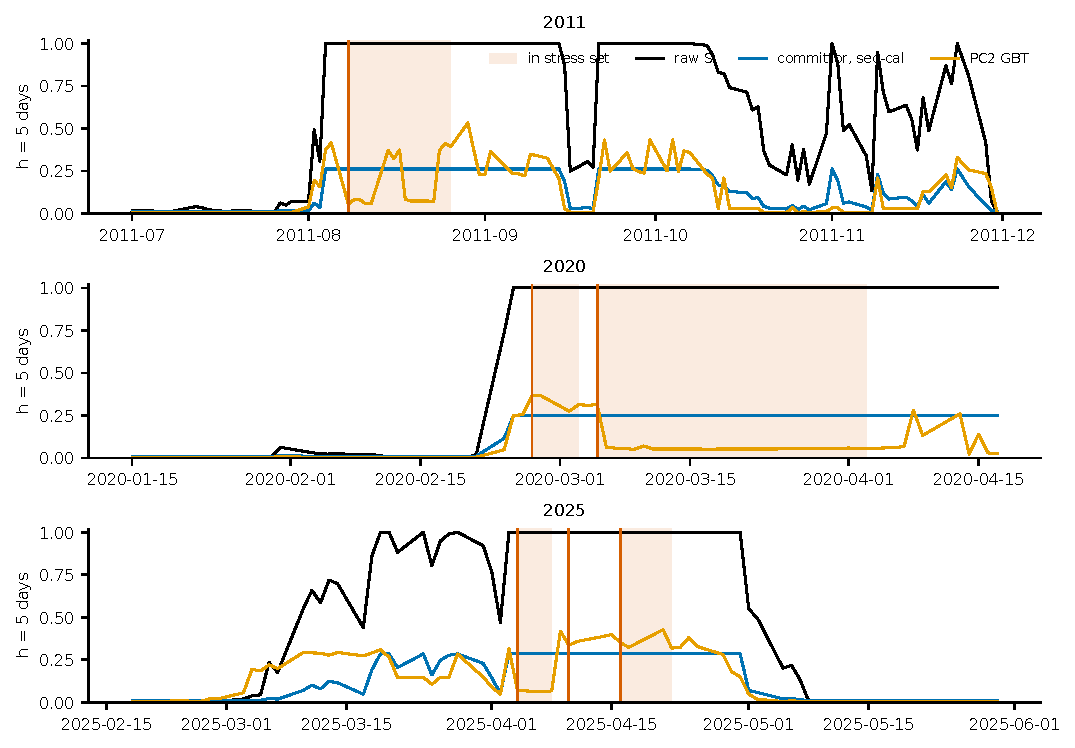
\includegraphics[width=\textwidth]{figures/fig5_cases.pdf}
\caption{Three episodes ($h=5$). Shaded, days in the stress set; vertical lines, entries. Data: P2\_F5\_case\_series.csv.}\label{fig:cases}\end{figure}

\section{An unseen era and two other markets}\label{sec:markets}
The protocol transfers without change to an era and to markets it has never seen, and there the 20-day advantage of the raw score disappears. The first out-of-sample year of each extension was fixed before any result by one rule, the first calendar year with at least 1,000 training rows: \FirstOOSEra for the S\&P~500 archive, \FirstOOSBTC for Bitcoin and \FirstOOSETH for Ether. The same features, event rule and estimators reproduce the calibration picture: the raw score is badly miscalibrated---its BSS at 5 days in 1957--1999 is \BSSrawEraFive---and recalibration brings it to the level of the classifiers (Table~\ref{tab:markets}, Fig.~\ref{fig:markets}). No comparison with the recalibrated forecast is significant after Holm adjustment in any market. The paired DSC intervals of the raw score against logistic regression include zero at 20 days in all three samples, and at 5 days logistic regression discriminates better than the raw score in 1957--1999 and worse in Ether. The long era offers the most event episodes of any sample, \EpisEraFive at 5 days and \EpisEraTwenty at 20 days.

The era is also the one place where the evidence on drift is mixed: the quasi-binomial test rejects homogeneity of the saturated-day event rate at 5 days ($p=\,$\QBEraFive) and at 20 days ($p=\,$\QBEraTwenty), while the episode permutation test does not ($p=\,$\PermEraFive and \PermEraTwenty). The quasi-binomial test assumes a common dispersion for all episodes and the permutation test does not, and in samples like the headline one the quasi-binomial test is liberal (Section~\ref{sec:size}); we report both and read the era as weak evidence of drift at most.

\begin{table}[t]\centering\small
\caption{An unseen era and two other markets (common-7 state, expanding windows, first out-of-sample year by the rule of Section~\ref{sec:markets}). Homogeneity: saturated-day event rate across years; -- if fewer than two years have five saturated days.}\label{tab:markets}
\fittable{\begin{tabular}{llrrrrrr}\toprule
market & $h$ & \multicolumn{4}{c}{BSS} & $\Delta$DSC raw $S-$PC2 logistic & homogeneity $p$\\
\cmidrule(lr){3-6} & & raw $S$ & OU seq-cal & PC2 logistic & PC2 GBT & [90\% interval] & perm. / quasi-bin.\\\midrule
S\&P 500, 1957--1999 & 5 & $-8.297$ & $0.064$ & $0.072$ & $0.079$ & [-0.0017, -0.0002] & 0.37 / 0.013\\
 & 20 & $-3.286$ & $0.053$ & $0.078$ & $0.065$ & [-0.0020, +0.0007] & 0.67 / 0.033\\
Bitcoin, 2018--2026 & 5 & $-0.013$ & $0.075$ & $0.117$ & $0.135$ & [-0.0033, +0.0016] & 1.00 / 0.93\\
 & 20 & $0.105$ & $0.113$ & $0.155$ & $0.168$ & [-0.0070, +0.0070] & 0.67 / 0.57\\
Ether, 2021--2026 & 5 & $-0.675$ & $0.006$ & $0.002$ & $-0.007$ & [+0.0002, +0.0041] & --\\
 & 20 & $-0.432$ & $-0.009$ & $-0.011$ & $-0.048$ & [-0.0009, +0.0039] & --\\
\bottomrule\end{tabular}
}\end{table}

\begin{figure}[t]\centering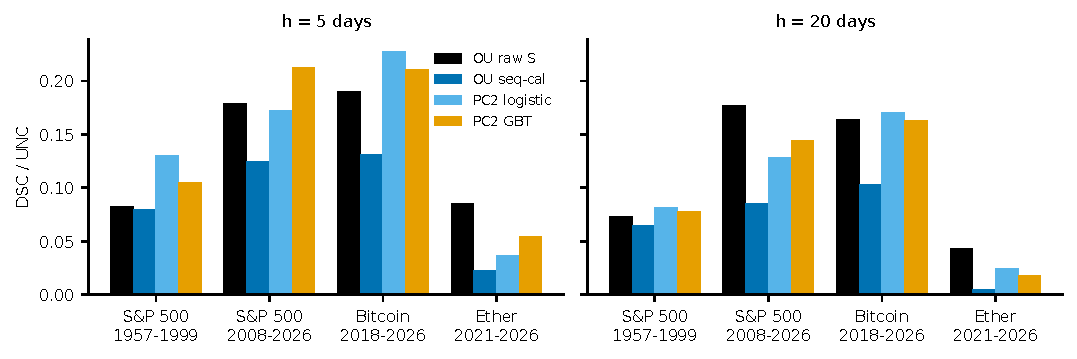
\includegraphics[width=\textwidth]{figures/fig6_markets.pdf}
\caption{Discrimination relative to uncertainty (DSC/UNC) by market. Data: P2\_X1\_decomposition.csv, P2\_F2\_decomposition\_exp.csv.}\label{fig:markets}\end{figure}

\section{Discussion}\label{sec:discussion}
For a user, a committor score is best read as the fitted model's probability of reaching its own learned region. It ranks days almost exactly as a single linear stress index does, it is not a probability of the operational event, and its saturation near one says little about how soon stress will follow. When a probability is needed, the score has to be recalibrated against the operational target, and it then performs like the recalibrated stress index and simple classifiers on the same information. The one advantage we found, more in-sample discrimination at 20 days than its own recalibration realizes, was confined to a single sample.

For evaluation, four practices follow, and none is specific to committors. The target should be stated: a score calibrated for the region it was built to reach can look badly miscalibrated for the event a user cares about, and the two diagnoses call for different remedies. Pooled AUCs of forecasts recalibrated year by year should not be reported; within-year AUCs can be (Table~\ref{tab:auc}). Inference should be carried out at the level of episodes: with \EpisMin to \EpisMax of them per sample, day-level tests manufacture drift and, among episode-level tests, permutation of whole episodes is the one that holds its size (Section~\ref{sec:size}); the absence of significant differences between forecasts is a statement about power as much as about the forecasts. And when the Giacomini--White test is used, a finite-memory version of the forecasts should be evaluated alongside the expanding one.

For the physics of the score, the comparison closes a loop with the companion paper. Trailing windows destroy transition information and add currents of their own; the forecasting state retains a genuine current, the leverage effect \citep{xingpan2026}. The committor computed from that state nevertheless ranks days as its projection on one direction does, so the current does not reach the forecasts.

The study has limits. It rests on one equity index at daily frequency, an earlier era of the same index and two cryptocurrencies; other equity indices were not available to us. The event rule and the recalibration link were fixed before the evaluation, and a detail of the rule---structurally zero labels in its first \LabelRows rows---changes no conclusion (Appendix~\ref{app:protocol}). The sequential recalibration uses past out-of-sample scores only, whereas the classifiers learn from all training labels; a calibration of the score on in-sample training labels, which would match their information, is not examined. Finally, with so few episodes the power to separate forecasts is low, which the model confidence set and the simulation make explicit.

\section{Conclusion}
A committor-type stress score forecasts entry into its own learned stress region, and it does so as a year-specific monotone transform of one linear stress index. For the operational event its numbers are not probabilities, and after recalibration it cannot be distinguished from the recalibrated index or from simple classifiers with the few independent episodes that daily data provide. Evaluated at that level, the apparent drift of its probability meaning disappears. Anyone who evaluates a warning of proximity to a learned region---in markets, ecosystems or the climate---should state its target, count episodes rather than days, and test at the level of episodes.

\section*{Data and code availability}
Anonymized data snapshots, scripts, all intermediate tables, figures and SHA-256 manifests are provided as supplementary material and will be deposited in a public archive upon acceptance. Every number in the text is generated by a script as a macro with its source (\texttt{manuscript\_p2/numbers\_sources.csv}), and \texttt{reproducibility\_p2/src/episode\_tests.py} provides the episode-level tests of Section~\ref{sec:drift} as a reusable function.

\section*{Declaration of generative AI and AI-assisted technologies in the writing process}
During the preparation of this work the authors used Claude (Anthropic) to edit the text and AI coding assistants to develop the analysis code. After using these tools, the authors reviewed and edited the content as needed; all numerical results were produced by the deposited, seeded scripts, and the authors take full responsibility for the content of the publication.

\section*{Declaration of competing interest}
The authors declare that they have no known competing financial interests or personal relationships that could have appeared to influence the work reported in this paper.

\section*{Funding}
This research did not receive any specific grant from funding agencies in the public, commercial, or not-for-profit sectors.

\section*{CRediT authorship contribution statement}
\textbf{Boyan Xing}: Conceptualization, Methodology, Software, Validation, Formal analysis, Investigation, Data Curation, Visualization, Writing -- Original Draft. \textbf{Jiayi Pan}: Writing -- Review \& Editing, Project Administration, Resources (financial and business interpretation of the forecasts).

\appendix
\section{Protocol details}\label{app:protocol}
The protocol is fixed before any evaluation. As a check of the implementation, forecasts recomputed by the present code from an archived 2000--2020 feature table coincide with the archived forecasts at stored precision (P2\_F1\_reproduction.csv). The lagged 1000-day volatility quantile of the stress rule needs 500 rows of history, so in the headline sample the labels of the first \LabelRows complete rows (\LabelFromDate to \LabelToDate) are structurally zero and enter every expanding training set. Dropping these rows changes the raw score and helps the classifiers slightly, but leaves the recalibrated committor forecast unchanged and makes no difference significant (Table~\ref{tab:labelrule}). The extension samples drop such rows by construction. Rolling-window comparisons are in Table~\ref{tab:rolling}, block-length sensitivity in Table~\ref{tab:blocks}, model-confidence-set $p$-values for all families in Table~\ref{tab:mcsall}, within-year AUCs in Table~\ref{tab:auc} and classifier settings in Table~\ref{tab:settings}.

\begin{table}[h]\centering\small
\caption{Label-rule sensitivity: headline protocol versus the same protocol without the \LabelRows rows with structurally zero labels. The interval quantile in the headline columns is that of Section~\ref{sec:murphy} (P2\_F2\_bootstrap\_exp.csv).}\label{tab:labelrule}
\fittable{\begin{tabular}{lrrrrrrrr}\toprule
 & \multicolumn{2}{c}{$h=5$, 2008--2026} & \multicolumn{2}{c}{$h=5$, 2009--2026} & \multicolumn{2}{c}{$h=20$, 2008--2026} & \multicolumn{2}{c}{$h=20$, 2009--2026}\\
quantity & headline & dropped & headline & dropped & headline & dropped & headline & dropped\\\midrule
BSS, OU seq-cal & $0.119$ & $0.118$ & $0.152$ & $0.151$ & $0.085$ & $0.087$ & $0.104$ & $0.105$\\
BSS, PC2 GBT & $0.195$ & $0.210$ & $0.181$ & $0.213$ & $0.151$ & $0.168$ & $0.125$ & $0.161$\\
BSS, PC2 logistic & $0.102$ & $0.113$ & $0.073$ & $0.086$ & $0.127$ & $0.137$ & $0.096$ & $0.118$\\
DSC, raw $S$ & $0.0058$ & $0.0058$ & $0.0047$ & $0.0047$ & $0.0144$ & $0.0143$ & $0.0103$ & $0.0108$\\
$\Delta$DSC raw $S-$seq-cal, q05 & $-0.0009$ & $-0.0007$ & $-0.0003$ & $-0.0003$ & $0.0010$ & $0.0016$ & $0.0002$ & $0.0005$\\
smallest Holm $p$ & 0.77 & 0.40 & 0.26 & 0.20 & 0.084 & 0.12 & 0.089 & 0.14\\
\bottomrule\end{tabular}
}\end{table}

\begin{table}[h]\centering\small
\caption{Difference in Brier skill (with 90\% interval, blocks of $2h$ days) and Holm-adjusted EWC $p$-value, rolling five-year windows.}\label{tab:rolling}
\resizebox{\textwidth}{!}{\begin{tabular}{lrrrrrrrr}\toprule
 & \multicolumn{2}{c}{$h=5$, 2008--2026} & \multicolumn{2}{c}{$h=5$, 2009--2026} & \multicolumn{2}{c}{$h=20$, 2008--2026} & \multicolumn{2}{c}{$h=20$, 2009--2026}\\
comparator & $\Delta$BSS & Holm $p$ & $\Delta$BSS & Holm $p$ & $\Delta$BSS & Holm $p$ & $\Delta$BSS & Holm $p$\\\midrule
MSM seq-cal & $0.005$ {\scriptsize[-0.011, +0.019]} & 1.00 & $0.006$ {\scriptsize[-0.015, +0.022]} & 1.00 & $-0.020$ {\scriptsize[-0.054, +0.005]} & 0.84 & $-0.024$ {\scriptsize[-0.068, +0.007]} & 0.53\\
AMC seq-cal & $-0.009$ {\scriptsize[-0.019, -0.002]} & 0.98 & $-0.012$ {\scriptsize[-0.024, -0.003]} & 0.65 & $-0.022$ {\scriptsize[-0.042, -0.005]} & 0.22 & $-0.026$ {\scriptsize[-0.052, -0.007]} & 0.21\\
PC2 logistic & $-0.005$ {\scriptsize[-0.082, +0.086]} & 1.00 & $-0.061$ {\scriptsize[-0.103, -0.017]} & 0.24 & $-0.018$ {\scriptsize[-0.099, +0.047]} & 0.84 & $-0.078$ {\scriptsize[-0.142, -0.020]} & 0.21\\
PC2 GBT & $0.061$ {\scriptsize[-0.014, +0.131]} & 1.00 & $0.012$ {\scriptsize[-0.052, +0.071]} & 1.00 & $0.056$ {\scriptsize[-0.030, +0.124]} & 0.84 & $0.012$ {\scriptsize[-0.062, +0.073]} & 0.77\\
raw logistic & $-0.012$ {\scriptsize[-0.086, +0.071]} & 1.00 & $-0.075$ {\scriptsize[-0.119, -0.031]} & 0.12 & $-0.122$ {\scriptsize[-0.239, -0.037]} & 0.19 & $-0.189$ {\scriptsize[-0.316, -0.116]} & 0.015\\
raw GBT & $-0.030$ {\scriptsize[-0.152, +0.062]} & 1.00 & $-0.066$ {\scriptsize[-0.202, +0.038]} & 1.00 & $-0.085$ {\scriptsize[-0.223, -0.002]} & 0.84 & $-0.143$ {\scriptsize[-0.306, -0.029]} & 0.21\\
\bottomrule\end{tabular}
}\end{table}

\begin{table}[h]\centering\scriptsize
\caption{Block-length sensitivity: 90\% moving-block-bootstrap intervals of the difference in Brier skill against the recalibrated committor forecast, expanding windows, for blocks of 5 to 60 days (1,000 resamples; the headline uses $2h$). Data: P2\_F4\_dbss.csv.}\label{tab:blocks}
\fittable{\begin{tabular}{llrrrrr}\toprule
comparator & $h$, sample & 5 days & 10 days & 20 days & 40 days & 60 days\\\midrule
MSM seq-cal & 5, 2008--2026 & [-0.015, +0.007] & [-0.015, +0.006] & [-0.014, +0.006] & [-0.014, +0.006] & [-0.014, +0.006]\\
 & 5, 2009--2026 & [-0.019, +0.008] & [-0.020, +0.006] & [-0.020, +0.004] & [-0.019, +0.002] & [-0.019, +0.002]\\
 & 20, 2008--2026 & [-0.031, -0.012] & [-0.032, -0.009] & [-0.035, -0.007] & [-0.040, -0.005] & [-0.042, -0.004]\\
 & 20, 2009--2026 & [-0.039, -0.014] & [-0.043, -0.012] & [-0.045, -0.011] & [-0.050, -0.010] & [-0.053, -0.005]\\
AMC seq-cal & 5, 2008--2026 & [-0.006, +0.006] & [-0.007, +0.006] & [-0.007, +0.007] & [-0.008, +0.006] & [-0.008, +0.005]\\
 & 5, 2009--2026 & [-0.007, +0.007] & [-0.009, +0.006] & [-0.011, +0.004] & [-0.011, +0.004] & [-0.012, +0.003]\\
 & 20, 2008--2026 & [-0.026, -0.011] & [-0.028, -0.010] & [-0.030, -0.009] & [-0.033, -0.007] & [-0.035, -0.006]\\
 & 20, 2009--2026 & [-0.033, -0.015] & [-0.035, -0.014] & [-0.038, -0.012] & [-0.042, -0.011] & [-0.042, -0.009]\\
PC2 logistic & 5, 2008--2026 & [-0.093, +0.064] & [-0.105, +0.083] & [-0.103, +0.074] & [-0.102, +0.075] & [-0.104, +0.067]\\
 & 5, 2009--2026 & [-0.118, -0.028] & [-0.123, -0.021] & [-0.122, -0.018] & [-0.124, -0.009] & [-0.121, -0.012]\\
 & 20, 2008--2026 & [+0.000, +0.086] & [-0.009, +0.094] & [-0.019, +0.102] & [-0.021, +0.109] & [-0.022, +0.114]\\
 & 20, 2009--2026 & [-0.038, +0.025] & [-0.042, +0.036] & [-0.044, +0.052] & [-0.046, +0.059] & [-0.053, +0.070]\\
PC2 GBT & 5, 2008--2026 & [+0.021, +0.130] & [+0.006, +0.137] & [+0.004, +0.137] & [+0.002, +0.134] & [+0.002, +0.131]\\
 & 5, 2009--2026 & [-0.005, +0.063] & [-0.010, +0.066] & [-0.017, +0.060] & [-0.014, +0.064] & [-0.016, +0.063]\\
 & 20, 2008--2026 & [+0.022, +0.107] & [+0.009, +0.111] & [+0.004, +0.110] & [-0.003, +0.114] & [-0.002, +0.116]\\
 & 20, 2009--2026 & [-0.007, +0.049] & [-0.009, +0.054] & [-0.014, +0.060] & [-0.018, +0.066] & [-0.024, +0.073]\\
raw logistic & 5, 2008--2026 & [-0.089, +0.053] & [-0.107, +0.068] & [-0.105, +0.076] & [-0.108, +0.080] & [-0.111, +0.074]\\
 & 5, 2009--2026 & [-0.130, -0.039] & [-0.134, -0.033] & [-0.135, -0.030] & [-0.133, -0.022] & [-0.132, -0.024]\\
 & 20, 2008--2026 & [-0.030, +0.045] & [-0.038, +0.056] & [-0.048, +0.060] & [-0.052, +0.064] & [-0.054, +0.068]\\
 & 20, 2009--2026 & [-0.063, +0.001] & [-0.072, +0.009] & [-0.076, +0.020] & [-0.080, +0.021] & [-0.087, +0.033]\\
raw GBT & 5, 2008--2026 & [-0.077, +0.063] & [-0.095, +0.079] & [-0.105, +0.081] & [-0.116, +0.079] & [-0.098, +0.069]\\
 & 5, 2009--2026 & [-0.117, +0.026] & [-0.130, +0.039] & [-0.145, +0.037] & [-0.144, +0.033] & [-0.155, +0.030]\\
 & 20, 2008--2026 & [-0.039, +0.070] & [-0.056, +0.075] & [-0.079, +0.085] & [-0.087, +0.085] & [-0.093, +0.087]\\
 & 20, 2009--2026 & [-0.076, +0.031] & [-0.096, +0.048] & [-0.119, +0.073] & [-0.128, +0.079] & [-0.149, +0.086]\\
\bottomrule\end{tabular}
}\end{table}

\begin{table}[h]\centering\small
\caption{Model-confidence-set $p$-values in all eight families (window scheme, horizon and sample 2008--2026 or 2009--2026; $T_{\max}$ statistic, blocks of $2h$ days). A model is in the 90\% set if its $p$-value is at least 0.10. Data: P2\_F4\_mcs.csv.}\label{tab:mcsall}
\fittable{\begin{tabular}{lrrrrrrrr}\toprule
 & \multicolumn{4}{c}{expanding windows} & \multicolumn{4}{c}{rolling five-year windows}\\
\cmidrule(lr){2-5}\cmidrule(lr){6-9} $h$ & 5 & 5 & 20 & 20 & 5 & 5 & 20 & 20\\
method & 08--26 & 09--26 & 08--26 & 09--26 & 08--26 & 09--26 & 08--26 & 09--26\\\midrule
OU seq-cal & 0.82 & 0.52 & 0.56 & 0.91 & 0.85 & 0.73 & 0.55 & 0.76\\
MSM seq-cal & 0.82 & 0.52 & 0.23 & 0.72 & 0.85 & 0.88 & 0.55 & 0.42\\
AMC seq-cal & 0.82 & 0.52 & 0.27 & 0.76 & 0.85 & 0.44 & 0.42 & 0.29\\
PC2 logistic & 0.82 & 0.18 & 0.65 & 0.91 & 0.85 & 0.28 & 0.55 & 0.15\\
PC2 GBT & 1.00 & 1.00 & 1.00 & 1.00 & 1.00 & 1.00 & 1.00 & 1.00\\
raw logistic & 0.76 & 0.085 & 0.56 & 0.72 & 0.85 & 0.15 & 0.034 & 0.030\\
raw GBT & 0.82 & 0.52 & 0.65 & 0.91 & 0.85 & 0.44 & 0.28 & 0.15\\
climatology & 0.013 & 0.015 & 0.079 & 0.21 & 0.002 & 0.001 & 0.015 & 0.030\\
\bottomrule\end{tabular}
}\end{table}

\begin{table}[h]\centering\small
\caption{Within-year AUC for the operational event, 2008--2026: median and quartiles over model years in which the forecast is not constant. Within a year a sequentially recalibrated forecast is a fixed increasing transform of its raw score and has the same AUC, so the rows of the raw scores also describe their recalibrated versions. Data: P2\_F2\_annual\_auc\_exp.csv.}\label{tab:auc}
\fittable{\begin{tabular}{lrrrr}\toprule
 & \multicolumn{2}{c}{$h=5$ days} & \multicolumn{2}{c}{$h=20$ days}\\
\cmidrule(lr){2-3}\cmidrule(lr){4-5} method & median [quartiles] & years & median [quartiles] & years\\\midrule
OU raw S & 0.826 [0.802, 0.960] & 10 & 0.729 [0.587, 0.884] & 10\\
MSM raw & 0.824 [0.741, 0.951] & 10 & 0.676 [0.589, 0.896] & 10\\
AMC raw & 0.845 [0.732, 0.952] & 10 & 0.688 [0.587, 0.892] & 10\\
PC2 logistic & 0.851 [0.796, 0.943] & 10 & 0.706 [0.574, 0.884] & 10\\
PC2 GBT & 0.881 [0.831, 0.956] & 10 & 0.698 [0.549, 0.902] & 10\\
raw logistic & 0.777 [0.732, 0.840] & 10 & 0.666 [0.545, 0.877] & 10\\
raw GBT & 0.857 [0.794, 0.923] & 10 & 0.720 [0.570, 0.840] & 10\\
\bottomrule\end{tabular}
}\end{table}

\begin{table}[h]\centering\small
\caption{Brier skill of the classifiers under alternative settings, expanding windows. Data: P2\_F2\_decomposition\_exp.csv.}\label{tab:settings}
\fittable{\begin{tabular}{lrrrr}\toprule
setting & $h=5$, 2008--2026 & $h=5$, 2009--2026 & $h=20$, 2008--2026 & $h=20$, 2009--2026\\\midrule
PC2 logistic, $C=1$ (headline) & $0.102$ & $0.073$ & $0.127$ & $0.096$\\
PC2 logistic, $C=0.1$ & $0.096$ & $0.073$ & $0.123$ & $0.096$\\
PC2 logistic, $C=10$ & $0.085$ & $0.073$ & $0.128$ & $0.096$\\
raw logistic, $C=0.2$ (headline) & $0.097$ & $0.063$ & $0.093$ & $0.072$\\
raw logistic, $C=0.1$ & $0.097$ & $0.063$ & $0.096$ & $0.075$\\
raw logistic, $C=1$ & $0.073$ & $0.063$ & $0.089$ & $0.068$\\
raw logistic, $C=10$ & $0.055$ & $0.063$ & $0.088$ & $0.067$\\
PC2 GBT, depth 2, 120 trees (headline) & $0.195$ & $0.181$ & $0.151$ & $0.125$\\
PC2 GBT, cross-validated & $0.179$ & $0.171$ & $0.155$ & $0.129$\\
raw GBT, depth 2, 120 trees (headline) & $0.116$ & $0.113$ & $0.105$ & $0.083$\\
raw GBT, cross-validated & $0.129$ & $0.140$ & $0.096$ & $0.088$\\
\bottomrule\end{tabular}
}\end{table}

\section{Inference}\label{app:inference}
\paragraph{Fixed-smoothing tests.} For a loss differential $d_t$ of length $T$, the equal-weighted-cosine variance uses $\nu=\lfloor0.4\,T^{2/3}\rfloor$ cosine projections of $d_t-\bar d$, and $\sqrt T\,\bar d/\hat\Omega^{1/2}$ is compared with Student's $t_\nu$ \citep{lazarus2018,coroneo2020}; Newey--West versions with lags $h-1$ and 20 are reported in the replication files \citep{newey1987}.
\paragraph{Conditional test.} With instruments $(1,d_{t-h})$ the statistic $T\,\bar Z^\top\hat\Omega^{-1}\bar Z$ is compared with $\chi^2_2$ \citep{giacomini2006}; an EWC version with the $F$ reference distribution is reported as well. The split of Section~\ref{sec:compare} regresses $d_t$ on $(1,d_{t-h})$ with a Newey--West variance (lag $h-1$) and tests each coefficient separately (\nolinkurl{P2_B5_gw_split.csv}).
\paragraph{Fluctuation test.} The statistic of \citet{giacomini2010} is the sum of $d_t$ over a rolling window of $m=0.3T$ days divided by $\hat\sigma\sqrt m$, with $\hat\sigma^2$ the Newey--West long-run variance of $d_t$ over the whole sample; its two-sided 5\% critical value, \GRcrit, is simulated from the supremum over $r\in[0.3,1]$ of $|W(r)-W(r-0.3)|/\sqrt{0.3}$ for a standard Brownian motion $W$ (\nolinkurl{P2_B5_fluctuation.csv}).
\paragraph{Model confidence set.} Brier losses of the reference, the six comparators and climatology; $T_{\max}$ statistic and moving-block bootstrap with blocks of $2h$ days \citep{hansen2011}.
\paragraph{Episode tests.} Saturated days are grouped into saturation episodes (runs no more than $h$ trading days apart, split at the annual re-estimation); years with fewer than five saturated days are dropped. The Pearson dispersion of the year rates is compared with its distribution under random permutation of year labels across episodes. The quasi-binomial test treats each episode as a binomial count with a common dispersion and compares the deviance reduction of a year effect with an $F$ distribution. The drift penalty compares CORP discrimination under one monotone map for all years with one map per year (\nolinkurl{P2_F3_drift_penalty_exp.csv}).
\paragraph{Size simulation.} For each horizon the simulation takes the number of model years with at least five saturated days, the number of saturation episodes, the number of scored saturated days and the pooled event rate from the headline sample. Every year has $1+\mathrm{Poisson}(E/K-1)$ episodes of geometric length, with the mean length calibrated so that the mean number of scored days per episode matches the data. With probability $\pi_y$ an episode is followed by an entry at a time drawn uniformly from its days $1,\dots,\ell+h$; a saturated day is labelled 1 if the entry falls within the next $h$ days, and days from the entry on are not scored. Under the null $\pi_y=\pi$, calibrated to the pooled rate; under the alternatives $\operatorname{logit}\pi_y=\operatorname{logit}\pi+\delta z_y$ with $z_y\sim N(0,1)$. The permutation test uses 499 permutations (\nolinkurl{P2_S1_size_simulation.py}, seed 20261027).

\section{Data provenance}\label{app:data}
The S\&P~500 file is the gated file of the companion paper. Yahoo's volume of zero on 24 May 2023 is replaced by $3.739\times10^9$ shares ($3739.16\times10^4$ lots of 100 shares) reported by Tonghuashun, whose open, high, low and close for that day and whose volumes on the adjacent days coincide with Yahoo's; the companion paper shows that replacing it by the mean volume of the adjacent days changes none of its results. A copy of the download with that day deleted was not used, because dropping a trading day merges two daily returns and shifts every trailing window. The 1950--1999 archive agrees with the snapshot on all common days to 2018. Coin Metrics data start on 1 January 2013 (Bitcoin) and 1 March 2016 (Ether).

\bibliographystyle{elsarticle-harv}
\bibliography{refs}
\end{document}
